\chapter{RIP and EIGRP}\label{rip-and-eigrp}

\section{Routing Information Protocol
(RIP)}\label{routing-information-protocol-rip}

\begin{itemize}
\tightlist
\item
  Routing Information Protocol (Industry Standard)
\item
  is a DISTANCE VECTOR IGP

  \begin{itemize}
  \tightlist
  \item
    uses Routing-By-Rumor logic to learn/share routes
  \end{itemize}
\item
  Uses HOP COUNT as it's METRIC (One Router = One Hop) Bandwidth is
  irrelevant
\item
  MAX HOP COUNT is 15 (anything more is considered unreachable)
\item
  Has THREE VERSIONS:

  \begin{itemize}
  \tightlist
  \item
    RIPv1 and RIPv2; used for IPv4
  \item
    RIPng (RIP Next Generation) used for IPv6
  \end{itemize}
\item
  Uses TWO MESSAGE TYPES:

  \begin{itemize}
  \tightlist
  \item
    REQUEST :

    \begin{itemize}
    \tightlist
    \item
      To ask RIP-ENABLED neighbour ROUTERS to send their ROUTING TABLE
    \end{itemize}
  \item
    RESPONSE:

    \begin{itemize}
    \tightlist
    \item
      To SEND the LOCAL router's ROUTING TABLE to neighbouring ROUTERS
    \end{itemize}
  \end{itemize}
\end{itemize}

By DEFAULT, RIP-Enabled ROUTERS will share their ROUTING TABLE every 30
seconds

RIPv1 and RIPv2

RIPv1:

\begin{itemize}
\tightlist
\item
  Only advertises \emph{classful addresses} (Class A, Class B, Class C)
\item
  Doesn't support VLSM, CIDR
\item
  Doesn't include SUBNET MASK information in ADVERTISEMENTS (RESPONSE
  messages)

  \begin{itemize}
  \tightlist
  \item
    Example:

    \begin{itemize}
    \tightlist
    \item
      10.1.1.0/24 will become 10.0.0.0 (Class A Address, so assumed to
      be /8)
    \item
      172.16.192.0/18 will become 172.16.0.0 (Class B Address, so
      assumed to be /16)
    \item
      192.168.1.40/30 will become 172.168.1.0 (Class C Address, so
      assumed to be /24)
    \end{itemize}
  \end{itemize}
\item
  Messages are BROADCAST to 255.255.255.255
\end{itemize}

RIPv2:

\begin{itemize}
\tightlist
\item
  Supports VLSM, CIDR
\item
  Includes SUBNET MASK information in ADVERTISEMENTS
\item
  Messages are \textbf{multicast} to 224.0.0.9

  \begin{itemize}
  \tightlist
  \item
    Broadcast Messages are delivered to ALL devices on the local network
  \item
    Multicast Messages are delivered only to devices to have joined that
    specific \textbf{\emph{multicast group}}
  \end{itemize}
\end{itemize}

\section{Configuring RIP}\label{configuring-rip}

\begin{figure}
\centering
\pandocbounded{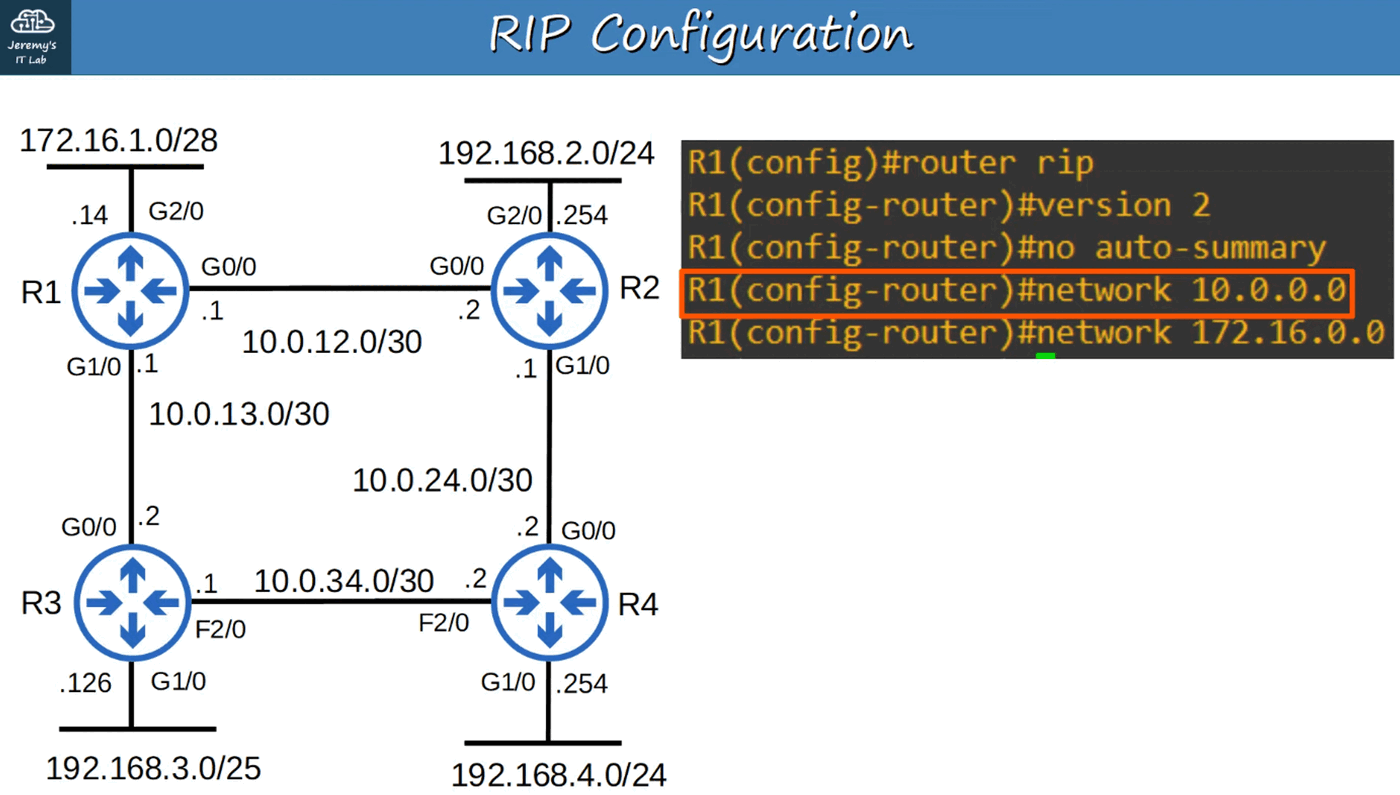
\includegraphics[keepaspectratio,alt={image}]{images/26-rip-and-eigrp/img-001.png}}
\end{figure}

The \textbf{``network''} command tells the router to:

\begin{itemize}
\tightlist
\item
  Look for INTERFACES with an IP ADDRESS that is in the specific RANGE
\item
  ACTIVATES RIP on the INTERFACES that fall in the RANGE
\item
  Form ADJACENCIES with connected RIP neighbors
\item
  Advertise the \textbf{NETWORK PREFIX of the INTERFACE} (NOT the prefix
  in the ``network'' command)
\end{itemize}

The OSPF and EIGRP \textbf{``network''} commands operate in the same way

Because the RIP ``network'' command is CLASSFUL. It will automatically
convert to CLASSFUL networks

\begin{itemize}
\tightlist
\item
  10.0.0.0 is assumed to be 10.0.0.0/8
\item
  R1 will look for ANY INTERFACES with an IP ADDRESS that matches
  10.0.0.0/8 (because it is /8 it only needs to match the FIRST 8 bits)
\item
  10.0.12.1 and 10.0.13.1 both match SO RIP is ACTIVATED on G0/0 and
  G0/1
\item
  R1 then forms ADJACENCIES with its neighbors R2 and R3
\item
  R1 ADVERTISES 10.0.12.0/30 and 10.0.13.0/30 (NOT 10.0.0.0/8) to it's
  RIP neighbors
\end{itemize}

\begin{figure}
\centering
\pandocbounded{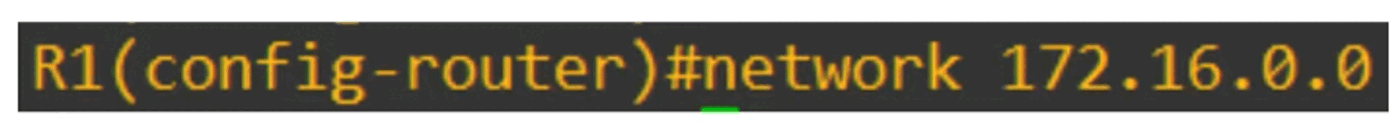
\includegraphics[keepaspectratio,alt={image}]{images/26-rip-and-eigrp/img-002.png}}
\end{figure}

\begin{itemize}
\tightlist
\item
  Because the ``network'' command is CLASSFUL, 172.16.0.0 is assumed to
  be 172.16.0.0/16
\item
  R1 will look for ANY INTERFACES that match 172.16.0.0/16
\item
  172.16.1.14 matches, so R1 will ACTIVATE RIP on G2/0
\item
  There are NO RIP neighbors connected to G2/0 so no NEW ADJACENCIES are
  formed

  \begin{itemize}
  \tightlist
  \item
    Although there are NO RIP neighbors, R1 will still send
    ADVERTISEMENTS out of G2/0.
  \item
    This is unnecessary traffic, so G2/0 should be configured as a
    \textbf{passive interface}
  \end{itemize}
\end{itemize}

\begin{figure}
\centering
\pandocbounded{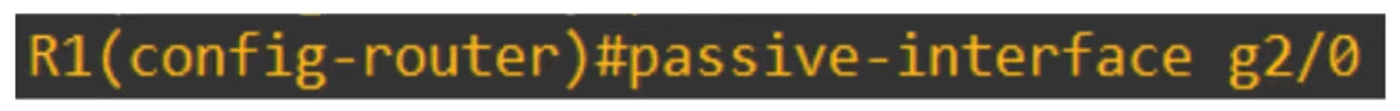
\includegraphics[keepaspectratio,alt={image}]{images/26-rip-and-eigrp/img-003.png}}
\end{figure}

\begin{itemize}
\tightlist
\item
  the ``passive-interface'' command tells the ROUTER to stop sending RIP
  advertisements out of the specified interface (G2/0)
\item
  However, the ROUTER will continue to ADVERTISE the network prefix of
  the interface (172.16.1.0/28) to it's RIP neighbors (R2, R3)
\item
  You should ALWAYS use this command on INTERFACES which don't have any
  RIP neighbors
\item
  EIGRP and OSPF both have the same passive INTERFACE functionality,
  using the same command.
\end{itemize}

\section{How to Advertise a Default Route into
RIP}\label{how-to-advertise-a-default-route-into-rip}

\begin{figure}
\centering
\pandocbounded{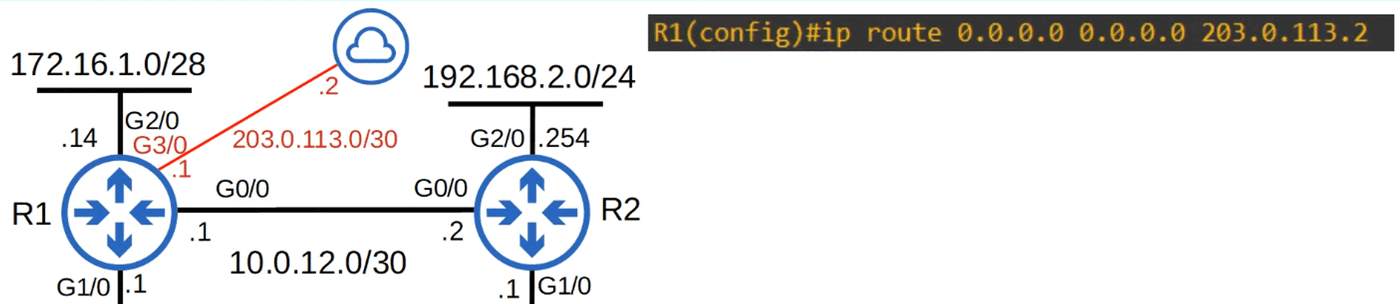
\includegraphics[keepaspectratio,alt={image}]{images/26-rip-and-eigrp/img-004.png}}
\end{figure}

\begin{figure}
\centering
\pandocbounded{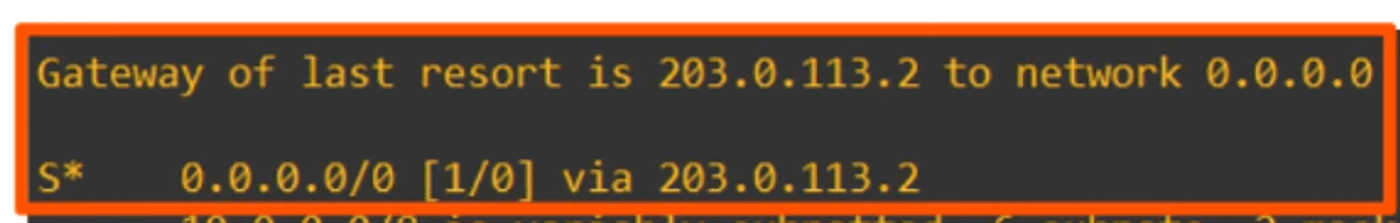
\includegraphics[keepaspectratio,alt={image}]{images/26-rip-and-eigrp/img-005.png}}
\end{figure}

To SHARE this DEFAULT ROUTE with R1's RIP neighbors, using this command:

\begin{figure}
\centering
\pandocbounded{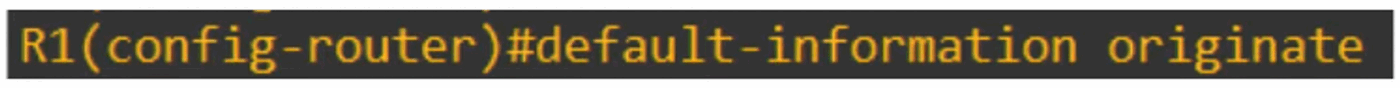
\includegraphics[keepaspectratio,alt={image}]{images/26-rip-and-eigrp/img-006.png}}
\end{figure}

RIP doesn't care about interface AD cost (RIP cost is 120), only
``hops''.

Since both have an equal number of ``hops'', both paths appear in the
DEFAULT ROUTE (Gateway of Last Resort)

\begin{figure}
\centering
\pandocbounded{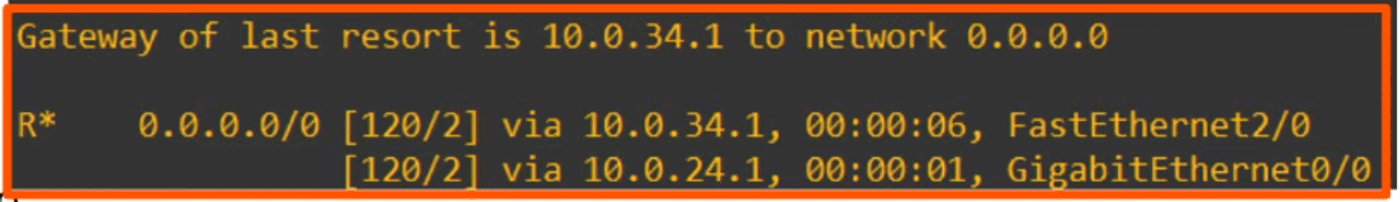
\includegraphics[keepaspectratio,alt={image}]{images/26-rip-and-eigrp/img-007.png}}
\end{figure}

``show ip protocols'' (for RIP)

\begin{figure}
\centering
\pandocbounded{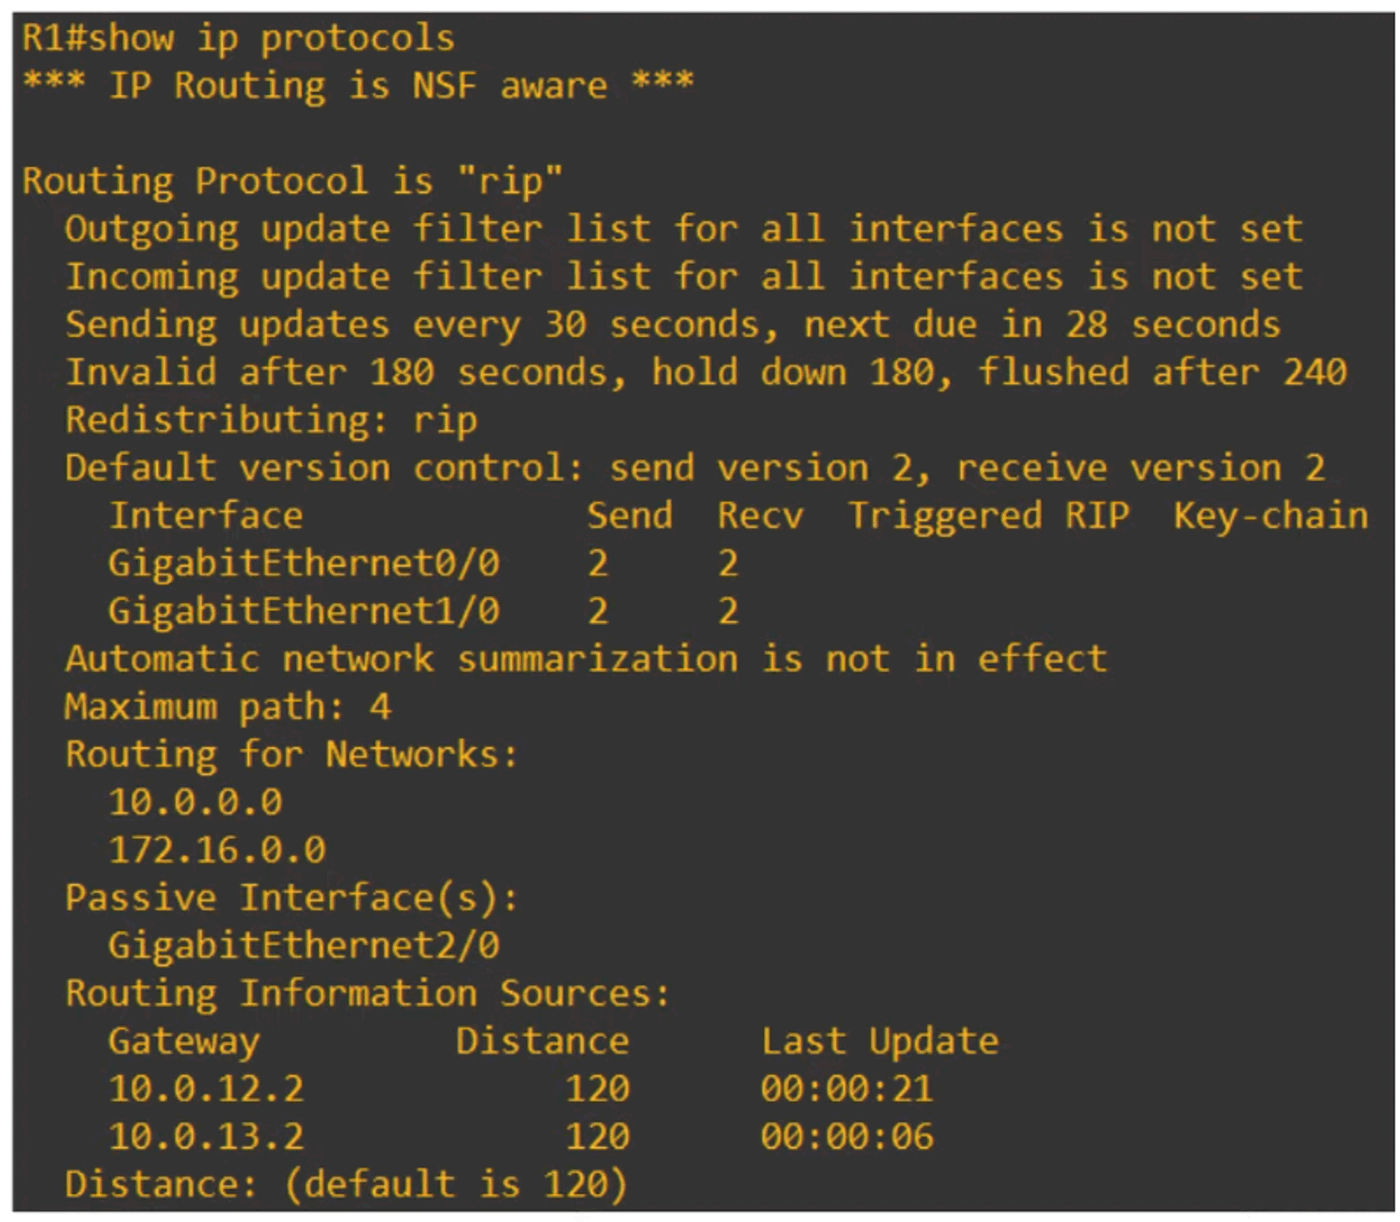
\includegraphics[keepaspectratio,alt={image}]{images/26-rip-and-eigrp/img-008.png}}
\end{figure}

``Maximum path: 4'' is the DEFAULT but can be changed with this command:

\begin{figure}
\centering
\pandocbounded{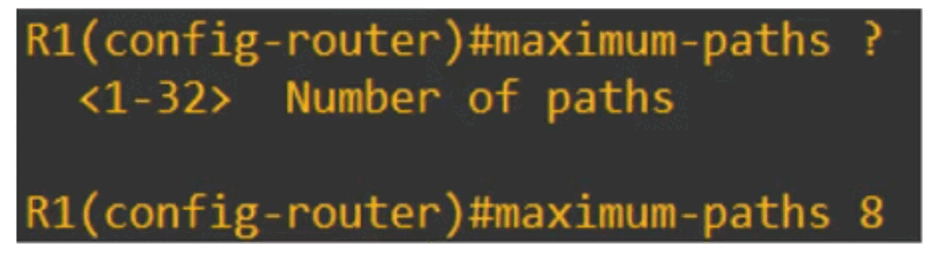
\includegraphics[keepaspectratio,alt={image}]{images/26-rip-and-eigrp/img-009.png}}
\end{figure}

``Distance'' (AD) can be changed with this command (DEFAULT is 120)

\begin{figure}
\centering
\pandocbounded{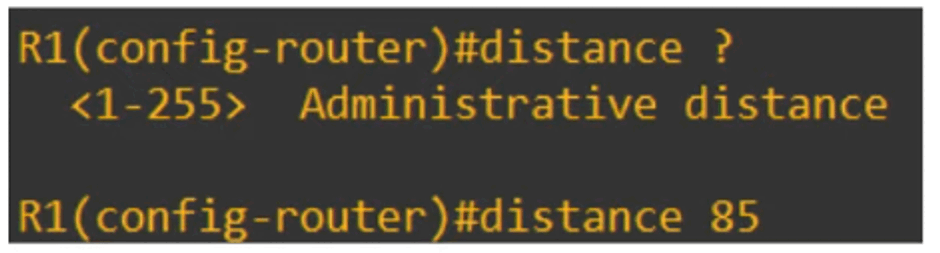
\includegraphics[keepaspectratio,alt={image}]{images/26-rip-and-eigrp/img-010.png}}
\end{figure}

\section{Enhanced Interior Gateway Routing Protocol
(EIGRP)}\label{enhanced-interior-gateway-routing-protocol-eigrp}

\begin{itemize}
\tightlist
\item
  Enhanced Interior Gateway Routing Protocol
\item
  is a DISTANCE VECTOR IGP
\item
  Was Cisco proprietary, but Cisco has now published it openly so other
  vendor can implement it on their equipment
\item
  Considered an ``advanced'' / ``hybrid'' DISTANCE VECTOR ROUTING
  PROTOCOL
\item
  Much faster than RIP in reacting to changes in the NETWORK
\item
  Does NOT have the 15 `hop count' limit of RIP
\item
  Sends messages using MULTICAST ADDRESS \textbf{224.0.0.10 (Memorize
  this number)}
\item
  Is the ONLY IGP that can perform \textbf{unequal}-cost load-balancing
  (by DEFAULT, it performs ECMP load-balancing over 4 paths like RIP)
\end{itemize}

\section{Configuration of EIGRP}\label{configuration-of-eigrp}

\begin{figure}
\centering
\pandocbounded{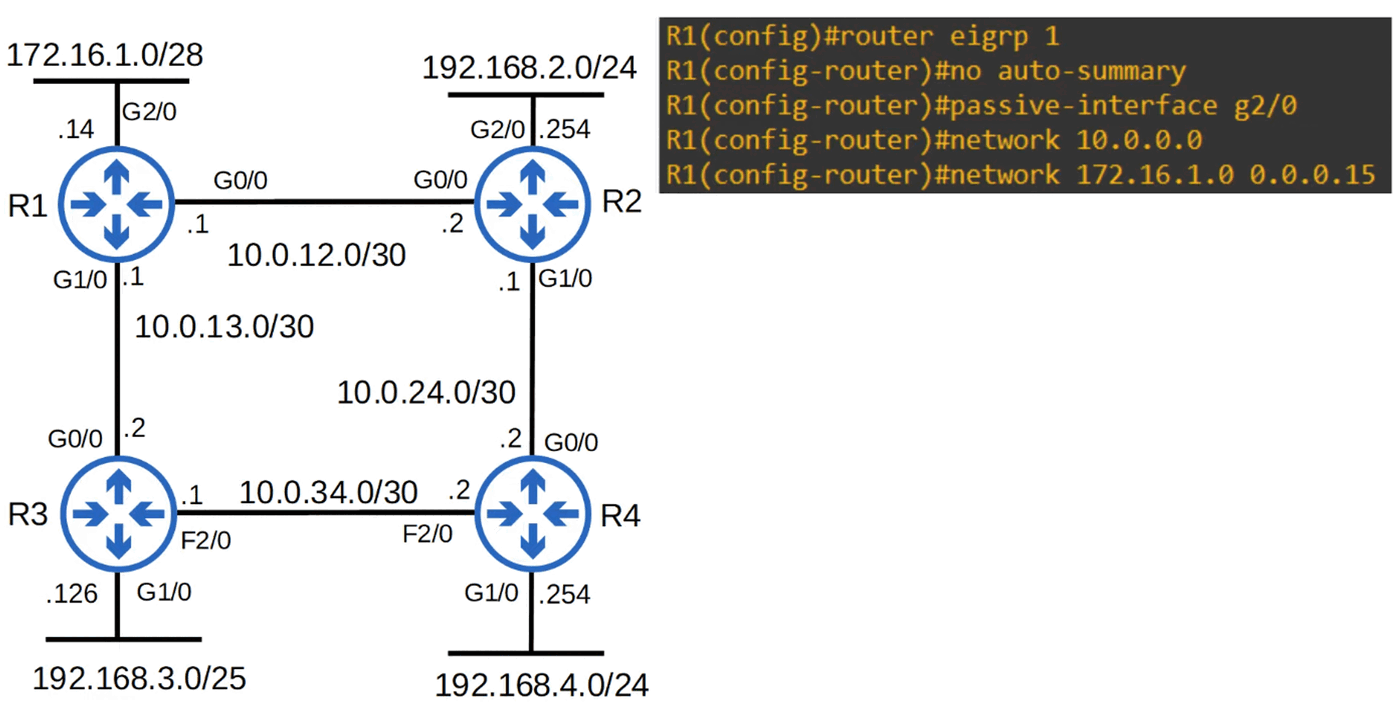
\includegraphics[keepaspectratio,alt={image}]{images/26-rip-and-eigrp/img-011.png}}
\end{figure}

``router eigrp \textless Autonomous System number\textgreater''

\begin{itemize}
\tightlist
\item
  The AS (Autonomous System) number MUST MATCH between ROUTERS or they
  will NOT form an ADJACENCY and share ROUTE information
\item
  Auto-summary might be ENABLED or DISABLED by DEFAULT; depending on the
  ROUTER/IOS version. If ENABLED, DISABLE it.
\item
  The \textbf{``network''} command will assume a CLASSFUL ADDRESS, if
  you don't specify the SUBNET MASK
\item
  EIGRP uses a \emph{wildcard mask} instead of a regular subnet mask
\end{itemize}

A WILDCARD MASK is an ``inverted'' SUBNET MASK

\begin{itemize}
\tightlist
\item
  All 1's in the SUBNET MASK are 0 in the equivalent WILDCARD MASK.
\item
  All 0s in the SUBNET MASK are 1 in the equivalent WILDCARD MASK.
\end{itemize}

\begin{figure}
\centering
\pandocbounded{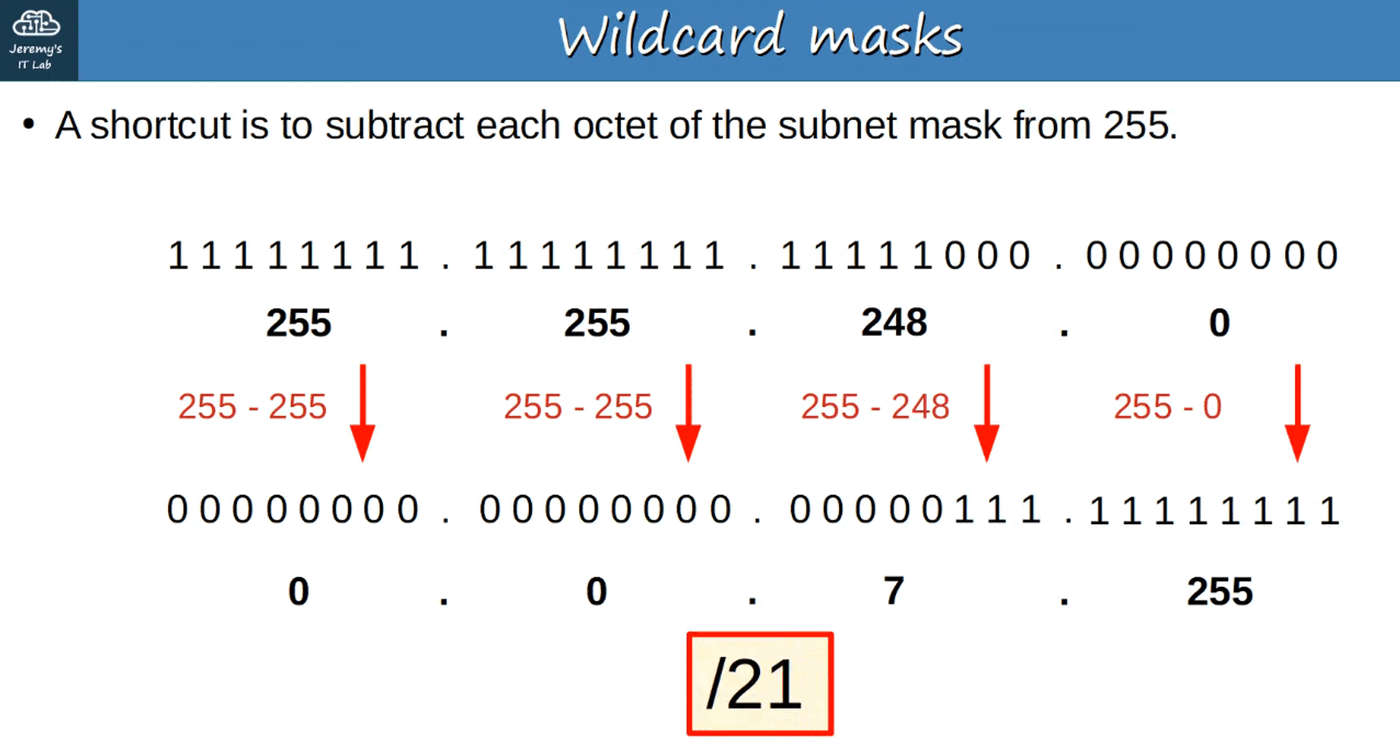
\includegraphics[keepaspectratio,alt={image}]{images/26-rip-and-eigrp/img-012.png}}
\end{figure}

``0'' in the WILDCARD MASK = BITS MUST MATCH !

``1'' in the WILDCARD MASK = Do not have to match

\begin{figure}
\centering
\pandocbounded{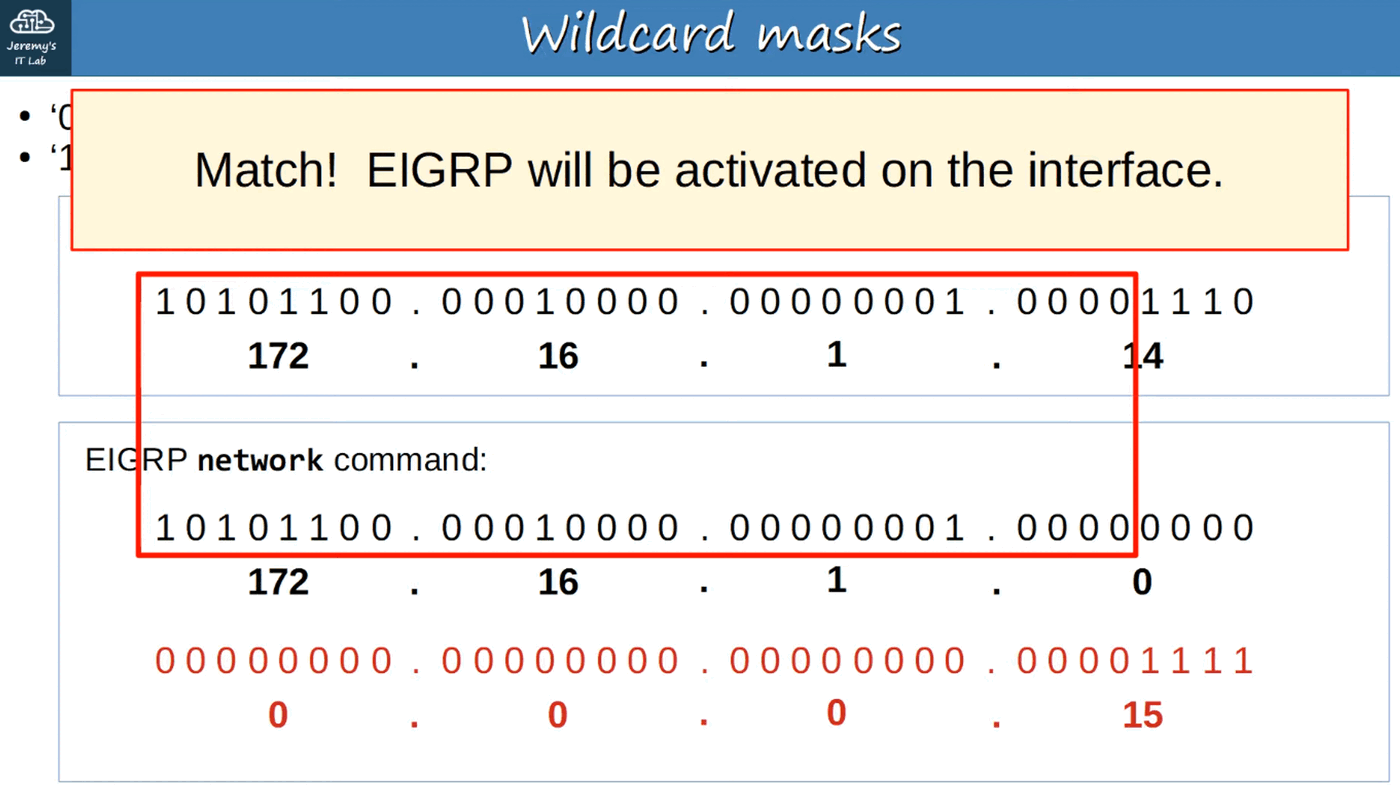
\includegraphics[keepaspectratio,alt={image}]{images/26-rip-and-eigrp/img-013.png}}
\end{figure}

\begin{figure}
\centering
\pandocbounded{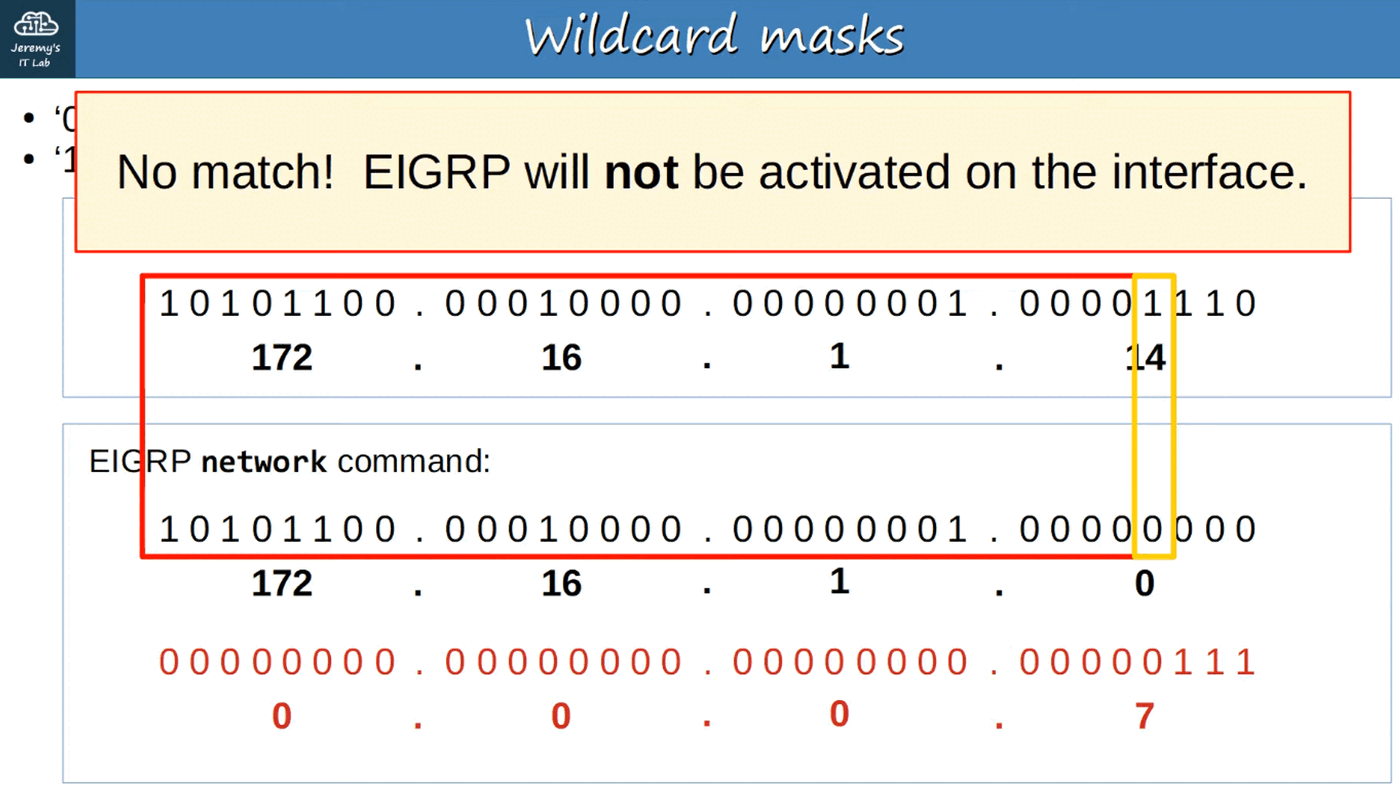
\includegraphics[keepaspectratio,alt={image}]{images/26-rip-and-eigrp/img-014.png}}
\end{figure}

\begin{figure}
\centering
\pandocbounded{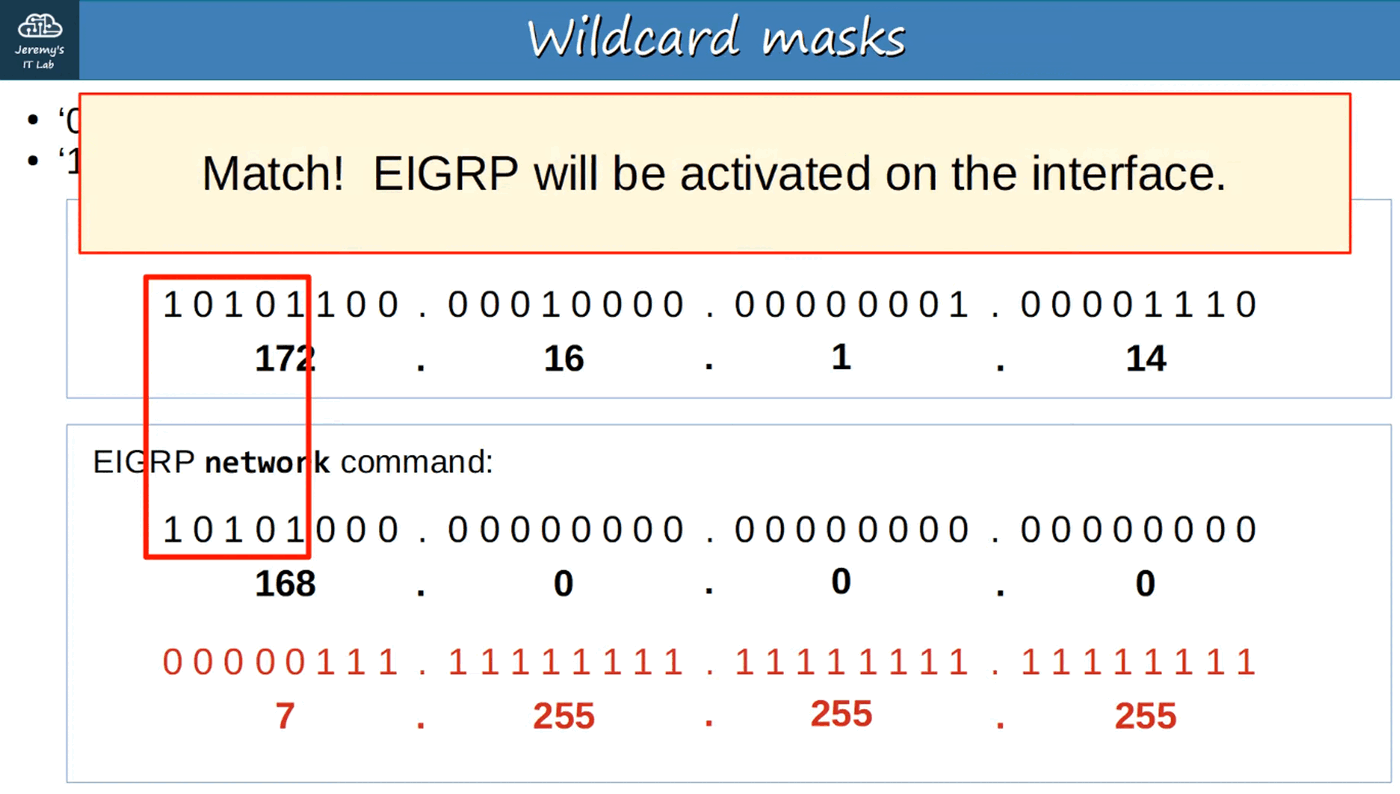
\includegraphics[keepaspectratio,alt={image}]{images/26-rip-and-eigrp/img-015.png}}
\end{figure}

``show ip protocols'' (for EIGRP)

\begin{figure}
\centering
\pandocbounded{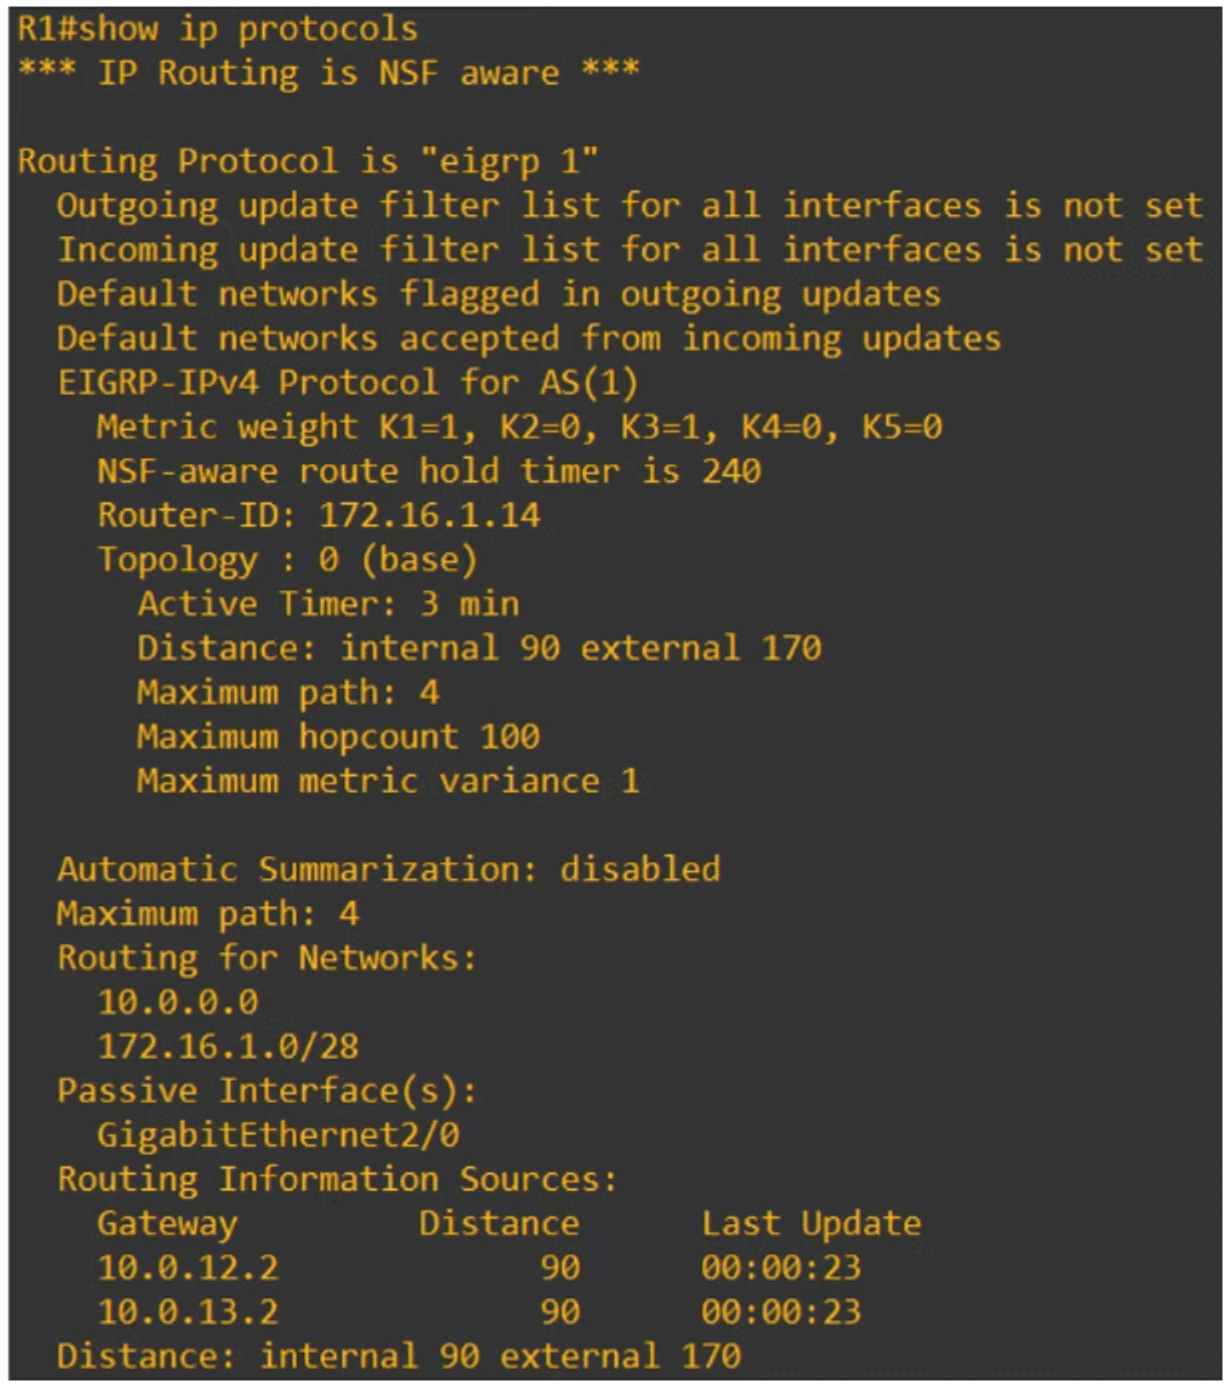
\includegraphics[keepaspectratio,alt={image}]{images/26-rip-and-eigrp/img-016.png}}
\end{figure}

``Router ID''

ROUTER ID order of priority:

\begin{itemize}
\tightlist
\item
  Manual configuration
\item
  Highest IP ADDRESS on a LOOPBACK INTERFACE
\item
  Highest IP ADDRESS on a PHYSICAL INTERFACE
\end{itemize}

\begin{figure}
\centering
\pandocbounded{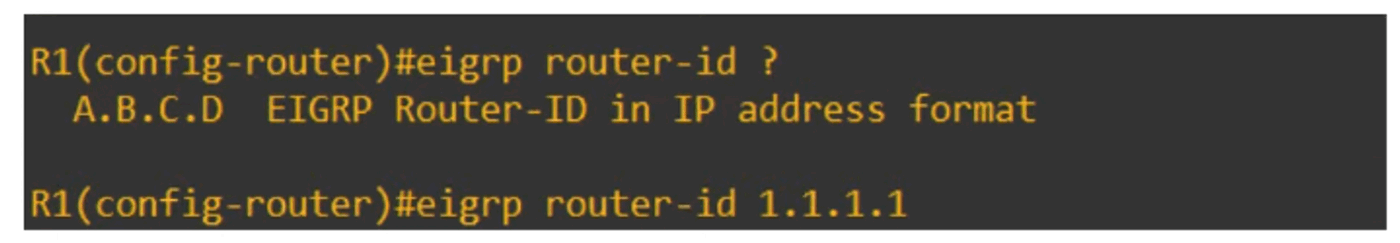
\includegraphics[keepaspectratio,alt={image}]{images/26-rip-and-eigrp/img-017.png}}
\end{figure}

``Distance'' (AD)

EIGRP has TWO VALUES:

\begin{itemize}
\tightlist
\item
  Internal = 90
\item
  External = 170
\end{itemize}

MEMORIZE THESE VALUES!

``show ip route'' (for EIGRP)

\begin{figure}
\centering
\pandocbounded{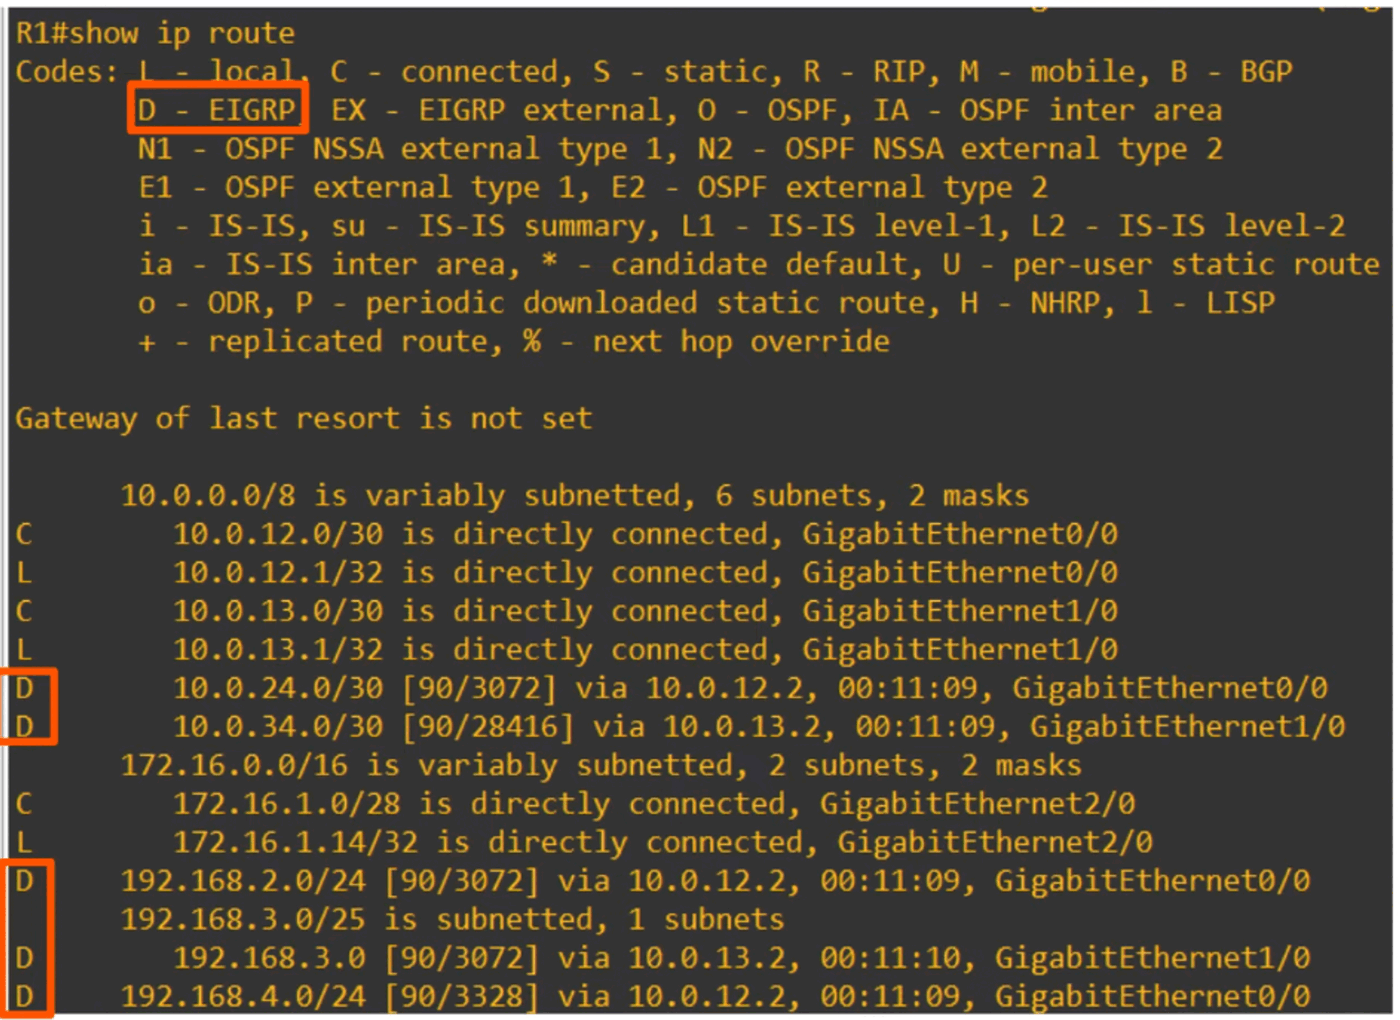
\includegraphics[keepaspectratio,alt={image}]{images/26-rip-and-eigrp/img-018.png}}
\end{figure}

NOTE the large METRIC numbers. This is a DOWNSIDE to EIGRP - even on
small networks!

\section{EIGRP Metric}\label{eigrp-metric}

\begin{itemize}
\tightlist
\item
  By DEFAULT, EIGRP uses BANDWIDTH and DELAY to calculate METRIC
\item
  Default ``K'' values are:

  \begin{itemize}
  \tightlist
  \item
    K1 = 1, K2 = 0, K3 = 1, K4 = 0, K5 = 0
  \end{itemize}
\end{itemize}

Simplified calculation : METRIC = BANDWIDTH (Slowest Link) + DELAY (of
ALL LINKS)

\section{EIGRP Terminology}\label{eigrp-terminology}

\begin{itemize}
\tightlist
\item
  \textbf{Feasible Distance} = This ROUTER's METRIC value to the ROUTE's
  DESTINATION
\item
  \textbf{Reported Distance} (aka \textbf{Advertised Distance}) = The
  neighbor's METRIC value to the ROUTE's DESTINATION
\end{itemize}

\begin{figure}
\centering
\pandocbounded{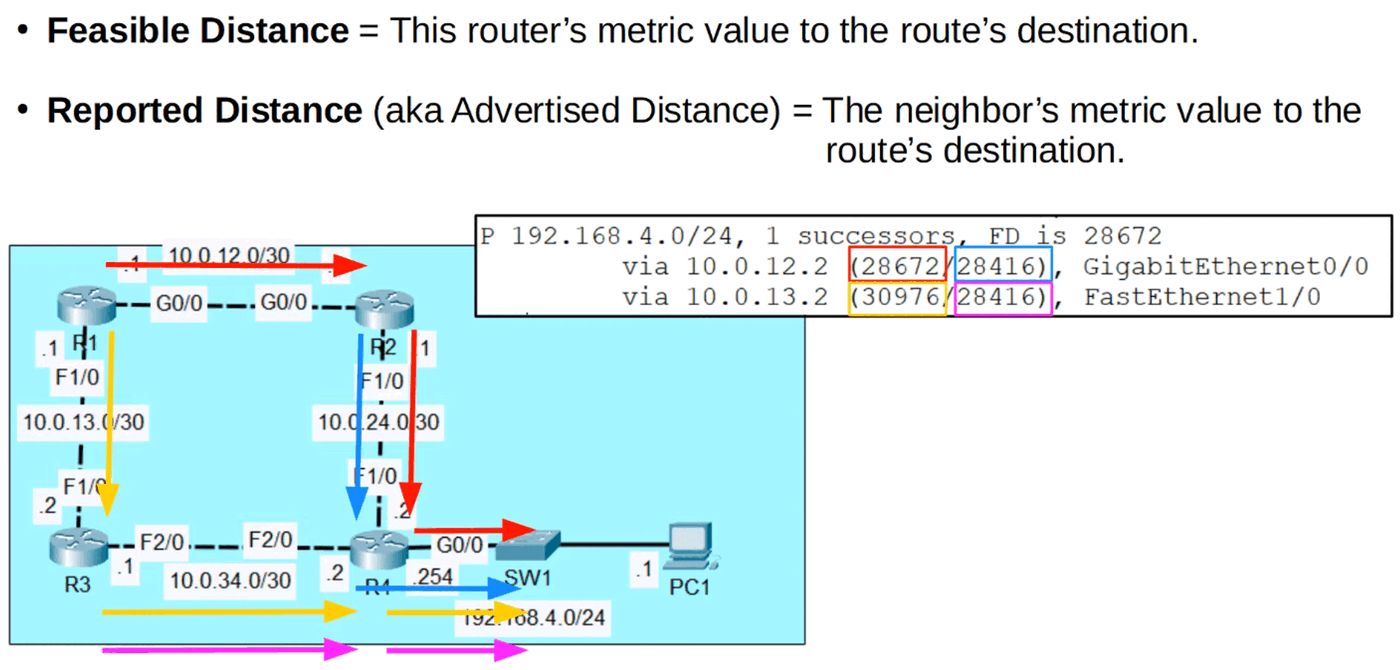
\includegraphics[keepaspectratio,alt={image}]{images/26-rip-and-eigrp/img-019.png}}
\end{figure}

\begin{itemize}
\tightlist
\item
  \textbf{Successor =} the ROUTE with the LOWEST METRIC to the
  DESTINATION (the best route)
\item
  \textbf{Feasible Successor} = An alternate ROUTE to the DESTINATION
  (not the best route) which meets the \emph{feasibility condition}
\end{itemize}

\textbf{FEASIBILITY CONDITION} : A ROUTE is considered a
\textbf{\emph{Feasible Successor}} if it's \textbf{\emph{Reported
Distance}} is LOWER than the Successor ROUTE's \textbf{\emph{Feasible
distance}}

\begin{figure}
\centering
\pandocbounded{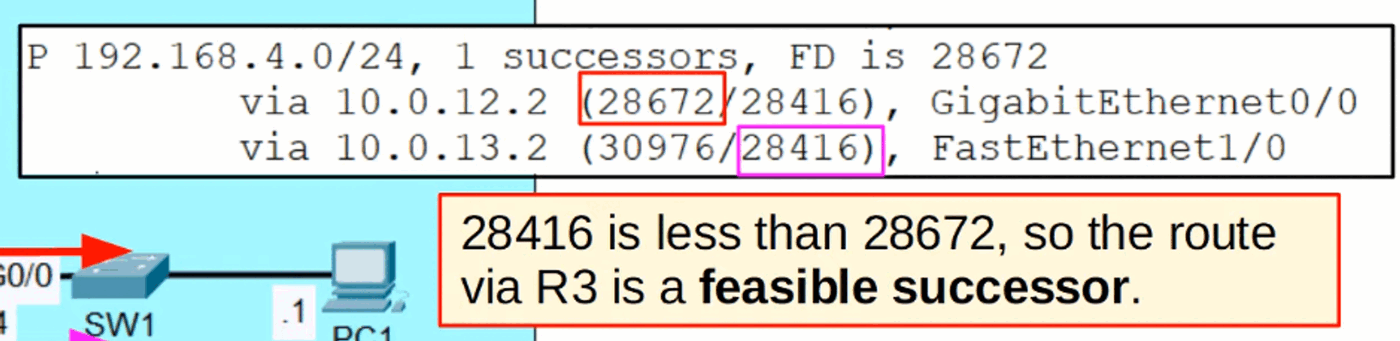
\includegraphics[keepaspectratio,alt={image}]{images/26-rip-and-eigrp/img-020.png}}
\end{figure}

\section{EIGRP : Unequal-Cost
Load-Balanced}\label{eigrp-unequal-cost-load-balanced}

\begin{figure}
\centering
\pandocbounded{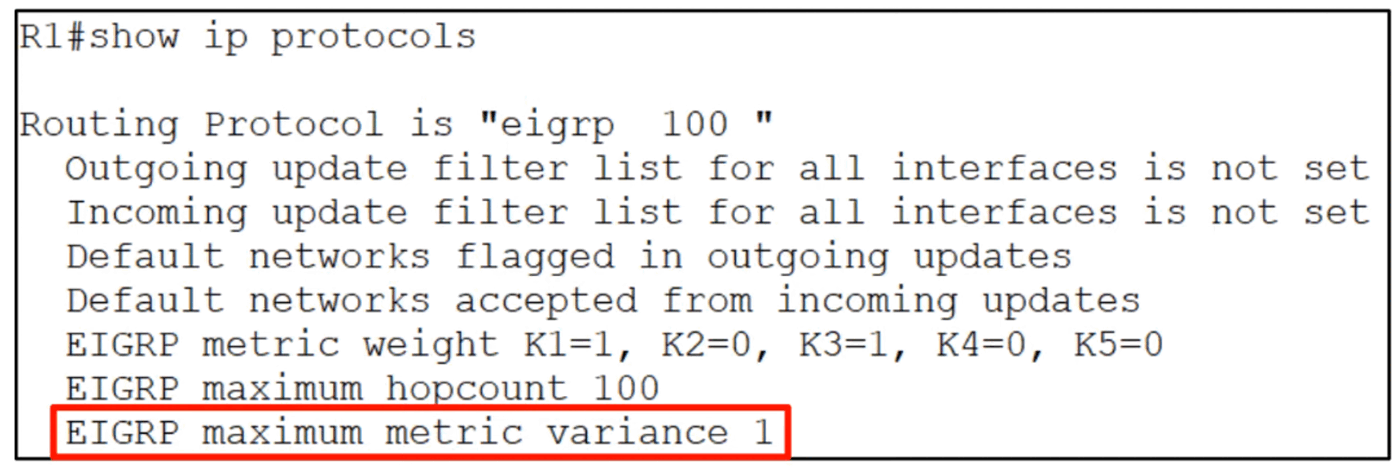
\includegraphics[keepaspectratio,alt={image}]{images/26-rip-and-eigrp/img-021.png}}
\end{figure}

``maximum metric variance 1'' = the DEFAULT value

Variance 1 = only ECMP (Equal-Cost Multiple Path) load-balancing will be
performed

\begin{figure}
\centering
\pandocbounded{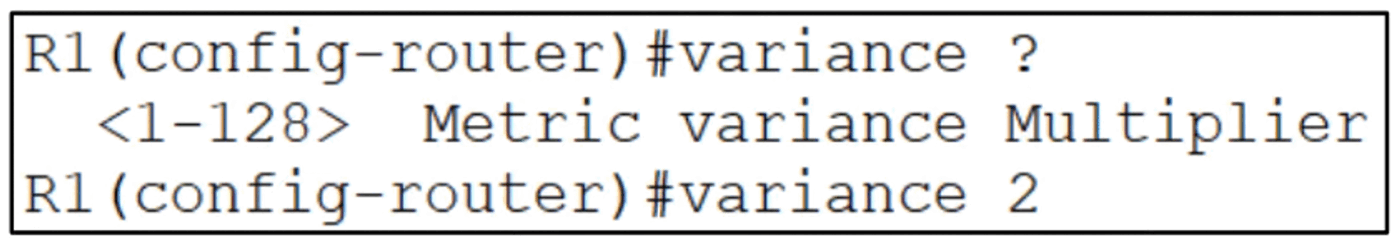
\includegraphics[keepaspectratio,alt={image}]{images/26-rip-and-eigrp/img-022.png}}
\end{figure}

Variance 2 = \textbf{\emph{feasible successor}} routes with an FD up to
2x the \textbf{\emph{successor}} route's FD can be used to load-balance

EIGRP will only perform UNEQUAL-COST LOAD-BALANCING over
\textbf{\emph{feasible successor}} ROUTES. If a ROUTE doesn't meet the
\textbf{\emph{feasibility condition}}, it will NEVER be selected for
load-balancing, regardless of \textbf{variance}
